% =====================================================================
% AI Academy -- National AI Center
% Software Engineering Final Project -- Team Presentation Deck
%
% HOW TO USE
% ----------
%   1. Edit the CONFIGURATION block (team name, topic, members).
%   2. Replace every \TODO{...} with your content. TODOs render in red,
%      so anything you forgot is visually obvious.
%   3. ~10 slides for a 10-minute talk. Roughly 1 min per slide; the
%      benchmark and architecture slides may take 2 min each.
%   4. Compile with pdfLaTeX (Overleaf works out of the box).
% =====================================================================

\PassOptionsToPackage{dvipsnames}{xcolor}
\documentclass[aspectratio=169,11pt]{beamer}

% ===== CONFIGURATION (edit these) ====================================
\newcommand{\teamname}{\TODO{Team Name}}
\newcommand{\topicchoice}{\TODO{Topic 1 / 2 / 3 / 4 -- Title}}
\newcommand{\memberone}{\TODO{Member A}}
\newcommand{\membertwo}{\TODO{Member B}}
\newcommand{\memberthree}{\TODO{Member C}}
\newcommand{\repolink}{\TODO{github.com/your-team/your-repo}}

\newcommand{\coursecode}{AI-ENG-110}
\newcommand{\coursename}{Software Engineering}
\newcommand{\institution}{AI Academy, National AI Center}
\newcommand{\semester}{Spring 2026}

% ===== PACKAGES ======================================================
\usepackage[T1]{fontenc}
\usepackage[utf8]{inputenc}
\usepackage{xcolor}
\usepackage{tabularx}
\usepackage{booktabs}
\usepackage{listings}
\usepackage{tikz}
\usetikzlibrary{shapes.geometric,arrows.meta,positioning,fit,backgrounds}

% ===== EARLY MACROS ==================================================
\definecolor{accent2}{HTML}{8B0000}
\newcommand{\TODO}[1]{\textcolor{accent2}{\textbf{[TODO: #1]}}}

% ===== BEAMER THEME (custom, no flashy decorations) =================
\usetheme{default}
\usefonttheme{professionalfonts}
\setbeamertemplate{navigation symbols}{}

\definecolor{accent}{HTML}{0B3D91}
\definecolor{soft}{HTML}{F2F4F8}
\definecolor{ok}{HTML}{166534}

\setbeamercolor{title}{fg=accent}
\setbeamercolor{frametitle}{fg=accent}
\setbeamercolor{section in head/foot}{bg=accent,fg=white}
\setbeamercolor{itemize item}{fg=accent}
\setbeamercolor{itemize subitem}{fg=accent}
\setbeamercolor{enumerate item}{fg=accent}
\setbeamercolor{block title}{bg=accent,fg=white}
\setbeamercolor{block body}{bg=soft,fg=black}

\setbeamerfont{title}{size=\Large,series=\bfseries}
\setbeamerfont{frametitle}{size=\large,series=\bfseries}
\setbeamerfont{footline}{size=\tiny}

% Footer with team + slide number
\setbeamertemplate{footline}{%
  \leavevmode%
  \hbox{\hspace*{2ex}\tiny\textit{\teamname{} -- \topicchoice}\hfill%
  \tiny\textit{\coursecode{} -- \semester{}}\hfill%
  \tiny\insertframenumber/\inserttotalframenumber\hspace*{2ex}}%
  \vskip1pt%
}

% ===== CODE LISTINGS =================================================
\definecolor{codegreen}{rgb}{0,0.55,0}
\definecolor{codepurple}{rgb}{0.55,0,0.78}
\lstdefinestyle{python}{
  language=Python,
  backgroundcolor=\color{soft},
  commentstyle=\color{codegreen},
  keywordstyle=\color{accent},
  stringstyle=\color{codepurple},
  basicstyle=\ttfamily\scriptsize,
  breaklines=true,
  frame=single,
  framerule=0.4pt,
  rulecolor=\color{black!30},
}

% =====================================================================
\begin{document}

% ========== SLIDE 1: TITLE ===========================================
{%
\setbeamertemplate{footline}{}
\begin{frame}[plain]
  \begin{center}
    \vspace{0.6cm}
    {\small \textsc{\institution}}\\[0.2em]
    {\small \textsc{\coursecode{} -- \coursename{} -- \semester{}}}\\[1.2em]
    \rule{0.7\textwidth}{0.6pt}\\[0.4em]
    {\Huge\bfseries\color{accent} \topicchoice}\\[0.4em]
    \rule{0.7\textwidth}{0.6pt}\\[1.2em]
    {\large \teamname}\\[0.6em]
    {\normalsize \memberone\quad\textbullet\quad\membertwo\quad\textbullet\quad\memberthree}\\[1cm]
    {\footnotesize\itshape Final Project Defense -- \TODO{Date}}\\[0.4em]
    {\footnotesize\texttt{\repolink}}
  \end{center}
\end{frame}
}

% ========== SLIDE 2: PROBLEM =========================================
\begin{frame}{The problem in one sentence}
  \begin{block}{What the system does}
    \TODO{One sentence stating the user problem and the system's contract. \\[3pt]
    Example: ``A user uploads a meal photo; we return calories, protein, carbs, and fat in under two seconds, citing the USDA entry for every ingredient.''}
  \end{block}

  \vspace{0.3em}
  \begin{columns}[T,onlytextwidth]
  \column{0.48\textwidth}
  \textbf{Inputs}
  \begin{itemize}
    \item \TODO{e.g.\ meal image (JPEG/PNG, $\le$5\,MB)}
    \item \TODO{e.g.\ user profile}
  \end{itemize}

  \column{0.48\textwidth}
  \textbf{Outputs}
  \begin{itemize}
    \item \TODO{e.g.\ structured JSON with per-ingredient kcal/protein/carbs/fat}
    \item \TODO{e.g.\ history record in SQLite}
  \end{itemize}
  \end{columns}

  \vspace{0.4em}
  \textbf{Entry points:} \TODO{CLI command + HTTP endpoint(s)}
\end{frame}

% ========== SLIDE 3: ARCHITECTURE ====================================
\begin{frame}{Architecture}
  \textbf{Module map.} The boundary between the \emph{provided} \texttt{ai/} package and \emph{our} SE layer is shown explicitly.

  \vspace{0.3em}
  \begin{center}
  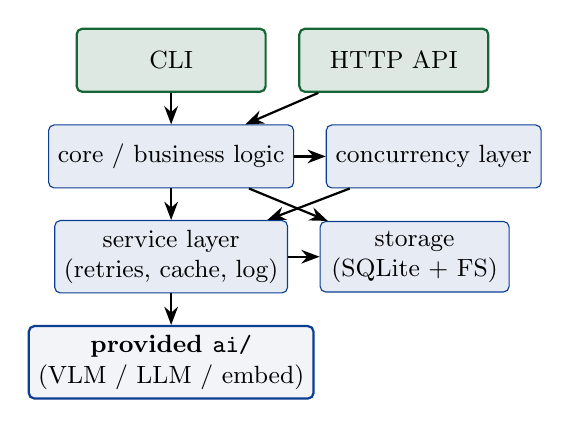
\begin{tikzpicture}[
    node distance=4mm,
    box/.style={draw,rounded corners=2pt,minimum width=2.4cm,minimum height=0.8cm,align=center,font=\small},
    aibox/.style={box,fill=soft,draw=accent,thick},
    sebox/.style={box,fill=accent!10,draw=accent},
    entry/.style={box,fill=ok!15,draw=ok,thick},
    arrow/.style={-Stealth,thick}
  ]
    % Entry points
    \node[entry] (cli) {CLI};
    \node[entry,right=of cli] (api) {HTTP API};

    % SE layer
    \node[sebox,below=of cli] (core) {core / business logic};
    \node[sebox,right=of core] (conc) {concurrency layer};
    \node[sebox,below=of core] (svc)  {service layer\\(retries, cache, log)};
    \node[sebox,right=of svc] (store) {storage\\(SQLite + FS)};

    % AI module
    \node[aibox,below=of svc] (ai) {\textbf{provided \texttt{ai/}}\\(VLM / LLM / embed)};

    % Arrows
    \draw[arrow] (cli) -- (core);
    \draw[arrow] (api) -- (core);
    \draw[arrow] (core) -- (conc);
    \draw[arrow] (core) -- (svc);
    \draw[arrow] (conc) -- (svc);
    \draw[arrow] (svc) -- (ai);
    \draw[arrow] (svc) -- (store);
    \draw[arrow] (core) -- (store);
  \end{tikzpicture}
  \end{center}

  \vspace{0.3em}
  {\footnotesize\textit{Replace this generic diagram with one specific to your team's modules.}}
\end{frame}

% ========== SLIDE 4: KEY DESIGN DECISIONS ============================
\begin{frame}{Three design decisions we can defend}
  \begin{enumerate}\setlength\itemsep{0.6em}
    \item \textbf{\TODO{Decision 1 (e.g.\ ``asyncio over threads'')}}\\
      \TODO{One-line justification + the alternative we rejected.}
    \item \textbf{\TODO{Decision 2 (e.g.\ ``Pydantic Settings over manual env parsing'')}}\\
      \TODO{One-line justification + trade-off accepted.}
    \item \textbf{\TODO{Decision 3 (e.g.\ ``SQLite + filesystem blobs over a single blob column'')}}\\
      \TODO{One-line justification + what would push us to change it.}
  \end{enumerate}

  \vspace{0.6em}
  \begin{block}{Expect to be asked}
    ``Why did you not use \TODO{the obvious alternative}?'' Have a 15-second answer ready for each of the three.
  \end{block}
\end{frame}

% ========== SLIDE 5: CONCURRENCY (THE BENCHMARK) =====================
\begin{frame}{Concurrency: the benchmark}
  \textbf{Workload:} \TODO{e.g.\ ``analyze 16 meals end-to-end on the developer laptop, fresh cache''}

  \vspace{0.4em}
  \begin{center}\small
  \begin{tabular}{lcc}
    \toprule
    & \textbf{Sequential} & \textbf{Concurrent (sem=10)} \\
    \midrule
    Wall-clock (s) & \TODO{42.1} & \TODO{7.3} \\
    Speedup        & 1.0$\times$ & \TODO{5.8$\times$} \\
    Provider 429s  & 0  & 0 \\
    \bottomrule
  \end{tabular}
  \end{center}

  \vspace{0.4em}
  \textbf{Bottleneck named:} \TODO{e.g.\ ``the embedding endpoint is dominant; the per-request RTT is ~70\,ms''}\\
  \textbf{What didn't reach $N\times$:} \TODO{e.g.\ ``USDA's free tier caps at 1000 req/h, so we bound the semaphore at 10''}

  \vspace{0.3em}
  {\footnotesize\textit{Numbers must reproduce from the README. Have the exact command line ready.}}
\end{frame}

% ========== SLIDE 6: ROBUSTNESS STORY ================================
\begin{frame}{Robustness: one concrete failure mode}
  \textbf{Scenario:} \TODO{e.g.\ ``the LLM returned valid JSON with \texttt{"meal\_recognized": true} but an empty ingredients list''}

  \vspace{0.3em}
  \textbf{How we surfaced it:} \TODO{e.g.\ a property-based test that fed random malformed bytes; manual chaos test that pulled the network mid-call.}

  \vspace{0.3em}
  \textbf{What the system does:}
  \begin{itemize}\setlength\itemsep{0.3em}
    \item \TODO{Retry: tenacity with exponential backoff (3 attempts, 1--8s).}
    \item \TODO{Validate: structured ``unknown meal'' response, not a 500.}
    \item \TODO{Log: \texttt{WARN ingredients\_empty image=... duration=...} with no PII.}
    \item \TODO{Degrade: HTTP returns 200 with an explicit \texttt{recognized=false} field.}
  \end{itemize}
\end{frame}

% ========== SLIDE 7: DEMO ============================================
\begin{frame}[fragile]{Live demo (or scripted demo)}
  \begin{block}{What we will run}
    \TODO{One sentence describing what the live demo shows.}
  \end{block}

  \vspace{0.4em}
  \textbf{Demo command (works inside Docker):}
  \begin{lstlisting}[style=python,language=bash,numbers=none]
$ docker run --env-file .env finalproj \
    python scripts/demo.py --input data/sample_meal.jpg
\end{lstlisting}

  \vspace{0.4em}
  \begin{itemize}
    \item \TODO{Bullet describing the most interesting on-screen output.}
    \item \TODO{Bullet calling out the timing improvement vs.\ sequential.}
  \end{itemize}

  \vspace{0.3em}
  {\footnotesize\textit{Have a pre-recorded screencast as backup in case the network is slow.}}
\end{frame}

% ========== SLIDE 8: TESTING =========================================
\begin{frame}{Testing}
  \begin{columns}[T,onlytextwidth]
  \column{0.55\textwidth}
  \textbf{Coverage \& shape}
  \begin{itemize}\setlength\itemsep{0.3em}
    \item Total coverage: \TODO{72}\,\%
    \item Provided \texttt{ai/} smoke tests: \textcolor{ok}{\textbf{passing}}
    \item Test count: \TODO{42 own + 28 smoke}
    \item All tests offline; AI module fully mocked
  \end{itemize}

  \column{0.42\textwidth}
  \textbf{Three tests worth calling out}
  \begin{itemize}\setlength\itemsep{0.3em}
    \item \TODO{Happy-path end-to-end}
    \item \TODO{Concurrency: one task raises, gather degrades}
    \item \TODO{Error path: provider 429 surfaces as retry}
  \end{itemize}
  \end{columns}

  \vspace{0.6em}
  \begin{block}{Tooling}
    \texttt{pytest} + \texttt{pytest-asyncio} + \texttt{pytest-cov} + \texttt{respx} / \texttt{unittest.mock}. \TODO{Add type-checker (mypy / pyright) result.}
  \end{block}
\end{frame}

% ========== SLIDE 9: LIMITATIONS + FUTURE ============================
\begin{frame}{Limitations \& what we'd do next}
  \textbf{Where the system is brittle today}
  \begin{itemize}\setlength\itemsep{0.3em}
    \item \TODO{e.g.\ no multi-provider failover; if Anthropic is down, we are.}
    \item \TODO{e.g.\ SQLite is single-writer; horizontal scaling needs Postgres.}
    \item \TODO{e.g.\ no rate-limit budget across processes (only within one).}
  \end{itemize}

  \vspace{0.4em}
  \textbf{Given another week we would}
  \begin{enumerate}\setlength\itemsep{0.3em}
    \item \TODO{e.g.\ add OpenTelemetry traces around every external call.}
    \item \TODO{e.g.\ load-test with k6 to find the real bottleneck.}
    \item \TODO{e.g.\ ship a Streamlit UI on top of the same business logic.}
  \end{enumerate}
\end{frame}

% ========== SLIDE 10: TEAM CONTRIBUTIONS =============================
\begin{frame}{Team contributions}
  \begin{center}\small
  \begin{tabularx}{\linewidth}{lXl}
    \toprule
    \textbf{Member} & \textbf{Primary ownership} & \textbf{Commits} \\
    \midrule
    \memberone   & \TODO{e.g.\ service layer, retries, config, CI}   & \TODO{34\%} \\
    \membertwo   & \TODO{e.g.\ HTTP API, concurrency, benchmark}    & \TODO{33\%} \\
    \memberthree & \TODO{e.g.\ storage, tests, Docker, report}      & \TODO{33\%} \\
    \bottomrule
  \end{tabularx}
  \end{center}

  \vspace{0.4em}
  \begin{block}{We can all answer:}
    Any of us can walk through any module on demand. Pick a file --- we'll defend it.
  \end{block}

  \vspace{0.4em}
  \textbf{AI tool use:} \TODO{One-sentence disclosure (e.g.\ ``Cursor scaffolded the FastAPI routes; we rewrote auth and validation.'').}
\end{frame}

% ========== SLIDE 11: THANK YOU / Q&A ================================
{%
\setbeamertemplate{footline}{}
\begin{frame}[plain]
  \begin{center}
    \vspace{1cm}
    {\Huge\bfseries\color{accent} Questions?}\\[1.2em]
    \rule{0.5\textwidth}{0.6pt}\\[1.2em]
    {\large \teamname}\\[0.6em]
    {\normalsize \texttt{\repolink}}\\[1cm]
    {\footnotesize\itshape ``We can walk through any file in the repo.''}
  \end{center}
\end{frame}
}

\end{document}
